%%%%%%%%%%%%%%%%%%%%%%%%%%%%%%%%%%%%%%%%%
% Structured General Purpose Assignment
% LaTeX Template
%
%
%%%%%%%%%%%%%%%%%%%%%%%%%%%%%%%%%%%%%%%%%

%----------------------------------------------------------------------------------------
%	PACKAGES AND OTHER DOCUMENT CONFIGURATIONS
%----------------------------------------------------------------------------------------

\documentclass[11pt,a4paper,titlepage]{article}


%\usepackage[utf8]{inputenc}
\usepackage{fontspec}
\usepackage{fancyhdr} % Required for custom headers
\usepackage{lastpage} % Required to determine the last page for the footer
\usepackage{extramarks} % Required for headers and footers
\usepackage{graphicx} % Required to insert images
\usepackage{lipsum} % Used for inserting dummy 'Lorem ipsum' text into the template
\usepackage{xltxtra}
\usepackage{amsmath}
\usepackage{amsfonts}
\usepackage{amssymb}
\usepackage{makeidx}
\usepackage{enumerate}
\usepackage{unicode-math}
\usepackage{caption}
\usepackage{subcaption}
\usepackage{algorithm}
\usepackage{algorithmic}
\usepackage[hidelinks]{hyperref}
\usepackage{grffile}
\usepackage{adjustbox}
\usepackage{wrapfig}
\usepackage{dirtree}
\usepackage{xfrac}
\usepackage{tikz}
\usepackage{tikz-qtree}
\usepackage{listings}

\usetikzlibrary{trees,calc,arrows.meta,positioning,decorations.pathreplacing,bending}

\input dirtree

\setmainfont[
UprightFont = Kerkis,
ItalicFont = KerkisItalics,
SlantedFont = KerkisItalics,
BoldFont = Kerkissb,               % Kerkisb
BoldItalicFont = Kerkissbi,        % Kerkisbi
BoldSlantedFont = Kerkissbi,       % Kerkisbi
SmallCapsFont = KerkisSmallCaps]   % KerkisSmallCaps-Bold for bold-face Small Caps
{Kerkis}

%\setmathfont{XITS Math}


% Margins
\topmargin=-0.45in
\evensidemargin=0in
\oddsidemargin=0in
\textwidth=6.5in
\textheight=9.15in
\headsep=0.25in 

\linespread{1.1} % Line spacing

% Set up the header and footer
\pagestyle{fancy}
\lhead{} % Top left header
\chead{\hmwkClass\ - \hmwkTitle} % Top center header
\rhead{\firstxmark} % Top right header
\lfoot{\lastxmark} % Bottom left footer
\cfoot{} % Bottom center footer
\rfoot{Σελίδα\ \thepage\ από\ \pageref{LastPage}} % Bottom right footer
\renewcommand\headrulewidth{0.4pt} % Size of the header rule
\renewcommand\footrulewidth{0.4pt} % Size of the footer rule

\setlength\parindent{0pt} % Removes all indentation from paragraphs

%----------------------------------------------------------------------------------------
%	DOCUMENT STRUCTURE COMMANDS
%	Skip this unless you know what you're doing
%----------------------------------------------------------------------------------------

\setcounter{secnumdepth}{0}
\setcounter{tocdepth}{1}

\DTsetlength{0.3em}{1.2em}{0.2em}{0.4pt}{0pt}
\newcommand*\rfrac[2]{{}^{#1}\!/_{#2}}

%----------------------------------------------------------------------------------------
%	LOCALIZATION
%----------------------------------------------------------------------------------------

\renewcommand\figurename{Σχήμα}
\renewcommand\contentsname{Περιεχόμενα}
\renewcommand\indexname{Ευρετήριο}
\renewcommand\tablename{Πίνακας}
\renewcommand\appendixname{Παράρτημα}

%----------------------------------------------------------------------------------------
%	NAME AND CLASS SECTION
%----------------------------------------------------------------------------------------

\newcommand{\hmwkTitle}{Εργασία 1} % Assignment title
\newcommand{\hmwkClass}{Παράλληλα \& Διανεμημένα Συστήματα} % Course/class
\newcommand{\hmwkAuthorName}{Δημανίδης Ιωάννης} % Your name
\newcommand{\hmwkAuthorAEM}{8358} % Your ΑΕΜ

%----------------------------------------------------------------------------------------
%	TITLE PAGE
%----------------------------------------------------------------------------------------

\title{
	\vspace{5cm}
	\huge{\textbf{\hmwkClass}}\\
	\vspace{9pt}
	\LARGE{\hmwkTitle}\\
	\vspace{7cm}
}

\author{\textbf{\hmwkAuthorName\ - \hmwkAuthorAEM}}
\date{} % Insert date here if you want it to appear below your name

%----------------------------------------------------------------------------------------

\begin{document}
	
	\maketitle
	
	%----------------------------------------------------------------------------------------
	%	TABLE OF CONTENTS
	%----------------------------------------------------------------------------------------
	
	%\setcounter{tocdepth}{1} % Uncomment this line if you don't want subsections listed in the ToC
	
	%\newpage
%	\tableofcontents
%	\clearpage
	%\newpage
	
	
	%----------------------------------------------------------------------------------------
	%	Document
	%----------------------------------------------------------------------------------------
	\section{Γενικά}
		Αρχικά εκτελούμε και τις δύο εκδοχές του αλγορίθμου \verb|bitonic sort|, imperative και recursive, για διάφορα μεγέθη εισόδου και παρατηρούμε ότι καθώς ανεβαίνουμε σε μέγεθος πίνακα το recursive version κάνει καλύτερο scale, καθώς έχει γρηγορότερους χρόνους εκτέλεσης από την imperative εκδοχή. Συνεπώς, είναι λογικό να παραλληλοποιήσουμε τον αναδρομικό \verb|bitonic sort| αλγόριθμο. Ορίζουμε λοιπόν το ακόλουθο project sructure:\\
		
		\begin{wrapfigure}{r}{0.4\textwidth}
			\begin{minipage}[t]{0.4\textwidth}
				\dirtree{%
					.1 trunk-gcc/.
					.2 bin/.
					.3 main.
					.2 build/.
					.3 bitonic\_cilk.o.
					.3 bitonic\_openmp.o.
					.3 bitonic\_pthread.o.
					.3 bitonic\_serial.o.
					.3 main.o.
					.2 include/.
					.3 bitonic\_cilk.h.
					.3 bitonic\_openmp.h.
					.3 bitonic\_pthread.h.
					.3 bitonic\_serial.h.
					.3 global\_vars.h.
					.3 main.h.
					.2 src/.
					.3 bitonic\_cilk.c.
					.3 bitonic\_openmp.c.
					.3 bitonic\_pthread.c.
					.3 bitonic\_serial.c.
					.3 main.c.
					.2 bench.rb.
					.2 makefile.
					.2 results.csv.
				}
			\end{minipage}
			\caption{Project Structure}			
		\end{wrapfigure}
		
		Ο φάκελος \verb|bin/| περιέχει το εκτελέσιμο αρχείο \verb|main|, το οποίο δέχεται δύο ορίσματα $q,p$ και εκτελεί όλες τις εκδοχές της \verb|bitonic sort| σε μέγεθος πίνακα $2^q$ με χρήση $2^p$ νημάτων και ελέγχει την ορθότητά τους. Αν όλες οι μέθοδοι ταξινομήσουν σωστά τον πίνακα τότε και μόνο τότε το πρόγραμμα επιστρέφει την τιμή \verb|EXIT_SUCCESS| στο κέλυφος, που ισοδυναμεί με 0, ειδάλλως επιστρέφει μια τιμή διάφορη του μηδενός. Η αρχικοποίηση και ο έλεγχος των πινάκων γίνεται με τη χρήση των δοσμένων συναρτήσεων \verb|init()|, και \verb|test()| αντίστοιχα.\\
		
		Στο φάκελο \verb|build/| βρίσκονται τα compiled object files από το κάθε αρχείο, τα οποιά αργότερα γίνονται linked μεταξύ τους και των βιβλιοθηκών του συστήματος για να παράξουν το \verb|main| εκτελέσιμο. Το directory \verb|include/| περιέχει τα header files για κάθε αρχείο κώδικα καθώς και το \verb|global_vars.h|, που περιέχει τα global variables του προγράμματος ώστε να είναι accessible από όλα τα άλλα αρχεία. Επιπλέον στον κατάλογο \verb|src/| περιέχονται όλα τα source files για κάθε διαφορετική υλοποίηση.\\

		Υπάρχουν επίσης τα αρχεία \verb|bench.rb, makefile, results.csv|, από τα οποία το πρώτο αποτελεί ένα Ruby script  το οποίο εκτελεί το πρόγραμμα \verb|main| για όλους τους πιθανούς συνδυασμούς των $q,p$ και καταγράφει τα αποτελέσματα στο CSV αρχείο \verb|results.csv|. Το αρχείο \verb|makefile| περιέχει οδηγίες για την εντολή \verb|make|, ώστε να γίνεται compile και link εύκολα όλο το πρόγραμμα, καθώς αποτελείται από πολλά αρχεία κατανεμημένα σε διάφο-ρους φακέλους.\\
		
		Τέλος να σημειωθεί ότι χρησιμοποιήθηκε η έκδοση \verb|4.8.1| του \verb|gcc|, και μάλιστα το \verb|cilkplus| branch, που υπήρχε στο directory \verb|/export/home/markioan/cilklpus-install/bin/gcc| με optimization level \verb|O3|. O λόγος που δεν χρησιμοποιήθηκε ο \verb|icc| είναι το γεγονός ότι εμφανι-ζόταν προβλήματα κατά το compilation και runtime των αρχείων \verb|bitonic_openmp.c| και \verb|bitonic_pthread.c|. Έτσι ήταν δυνατή η μεταγλώτιση μόνο των σειριακών υλοποιήσεων καθώς και της υλοποίησης με cilk. Όμως, δεδομένου ότι θα χρησιμοποιούσαμε διαφορετικούς compilers για διαφορετικά αρχεία δε θα είχαμε common point of reference όσον αφορά τα benchmarks, καθώς οι σειριακοί χρόνοι που αποτελούν το σημείο αναφοράς για τις διάφορες συγκρίσεις θα ήταν διαφορετικοί για τις ίδιες παραμέτρους του προβλήματος ανάλογα με το ποιος compiler χρησιμοποιήθηκε.

	\section{Παράλληλη υλοποίηση} 
		Όπως αναφέρθηκε και στην αρχή, παραλληλοποιούμε την αναδρομική εκδοχή του αλγο-ρίθμου διότι κάνει καλύτερα scale σε μεγάλα μεγέθη πίνακα από την imperative μορφή του, αλλά και γιατί είναι πιο εύκολο να υλοποιηθεί προγραμματιστικά, καθώς ουσιαστικά έχουμε μια συνάρτηση που καλεί πολλές φορές τον εαυτό της, και μάλιστα αυτές οι κλήσεις λειτουργούν σε δεδομένα ανεξάρτητα μεταξύ τους. Έτσι, αν κάθε φορά που η συνάρτηση \verb|bitonic sort| κάνει αναδρομική κλήση στον εαυτό της, κάνουμε spawn ένα thread, έχουμε παραλληλοποιήσει τον αλγόριθμο. Όπως είπαμε και πριν τα δεδομένα στα οποία θα λει-τουργεί κάθε νήμα θα είναι ανεξάρτητα μεταξύ τους αφού κάθε φορά η parent συνάρτηση θα καλεί δύο children, όπου το πρώτο παιδί θα λειτουργεί στο πρώτο μισό του πίνακα ενώ το δεύτερο παιδί θα λειτουργεί στο άλλο μισό. Η σχέση αυτή μπορεί να  περιγραφεί μαθηματικά ως εξής:
		\[T_s(n) = 2T_s\left(\rfrac{n}{2}\right) + T_m(n)\]
		Στη σχέση αυτή $T_s$ είναι ο χρόνος που θα κάνει η \verb|bitonic sort| σε βήματα, και $T_m$ ο αντίστοιχος χρόνος για τη \verb|bitonic merge|, η οποία λειτουργεί με αντίστοιχη λογική, οπότε παραλληλοποιείται εξίσου εύκολα. Η μαθηματική σχέση που περιγράφει την \verb|bitonic merge| είναι:
		\[T_m(n) = 2T_m\left(\rfrac{n}{2}\right) + \mathcal{O}\left(n\right)\]
		
		Όσον αφορά την υλοποίηση υπάρχουν 2 τρόποι: ο ένας τρόπος είναι κάθε φορά που η συνάρτηση καλεί τον εαυτό της, να δημιουργεί δύο νήματα, ένα για κάθε παιδί. Η εναλλα-κτική λύση είναι να κάνει spawn ένα thread για το πρώτο παιδί και το δεύτερο παιδί να το εκτελεί σειριακά. Με την πρώτη μέθοδο θα έχουμε πολλά idling threads τα οποία θα περιμένουν τα children τους να τελειώσουν με την εκτέλεση, πράγμα το οποίο είναι
		\begin{wrapfigure}{l}{0.35\textwidth}
			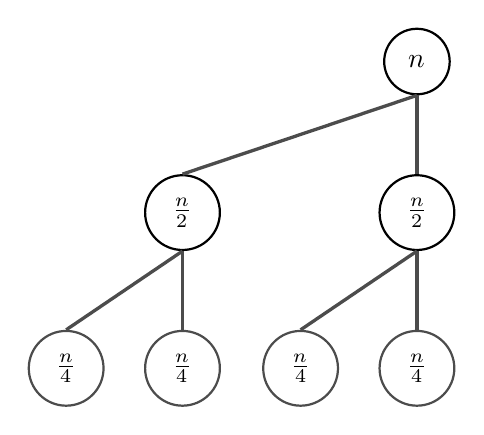
\begin{tikzpicture}
			[event/.style={circle,thick,draw,text width=0.5cm, text centered,font=\sffamily,anchor=north},
			edge from parent/.style={very thick,draw=black!70},
			]
			\node (g) [event] {$n$} 
			child {node[event,below= 1cm of g] (e1) {$\frac{n}{2}$}
				child {node[event,below= 1cm of e1] (e11) {$\frac{n}{4}$}}
				child {node[event,left= 0.5cm of e11] (e12) {$\frac{n}{4}$}}
			}
			child {node[event,left= 2cm of e1] (e2) {$\frac{n}{2}$}
				child {node[event,below= 1cm of e2] (e21) {$\frac{n}{4}$}}
				child {node[event,left= 0.5cm of e21] (e22) {$\frac{n}{4}$}}
			};
			\end{tikzpicture}
			\caption{Δένδρο αναδρομής}			
		\end{wrapfigure}
		ανεπιθύμητο, εκτός αν 	εφαρμοστεί κάποιου είδους job-stealing. Με την άλλη μέθοδο, δε θα υπάρχουν threads που θα περιμένουν, καθώς όταν ένα νήμα θα δημιουργεί ένα άλλο, θα συνεχίζει κανονικά την εκτέλεση του αντί να καλέσει ένα ακόμη νήμα και να περιμένει την περάτωση και των δύο child threads του. Και στις δύο περιπτώσεις ο αριθμός των νημάτων που θα είναι active κάθε φορά θα είναι ο ίδιος, απλά στη δεύτερη περίπτωση δε θα έχουμε idle threads. Το δέντρο αναδρομής με το μέγεθος του πίνακα σύμφωνα με αυτήν την υλοποίηση φαίνεται στο σχήμα. Όπου υπάρχει κάθετη γραμμή το κάθε thread συνεχίζει σειριακά, ενώ οι πλάγιες γραμμές δηλώνουν ότι έγινε spawn ένα νέο νήμα. Με την πρώτη, naive υλοποίηση κάθε κόμβος στο δέντρο αποτελεί ένα thread, αλλά μόνο τα φύλλα στο τελευταίο επίπεδο του δέντρου είναι active, όλα τα άλλα είναι idlers, περιμένοντας τα children τους να τελειώσουν. Με τη δεύτερη προσέγγιση, υπάρχουν τόσα threads όσα είναι και τα φύλλα του δέντρου. Τα παραπάνω μπορούν να διατύπωθουν και μαθηματικά ως εξής: στην πρώτη υλοποίηση έχουμε συνολικά $\sum_{i=0}^{k}2^i$ νήματα, όπου $k$ το επίπεδο του δέντρου αναδρομής στο οποίο βρισκόμαστε, από τα οποία τα $2^k$ είναι active ενώ τα υπόλοιπα $\sum_{i=0}^{k-1}2^i$ νήματα είναι idle. Με την δεύτερη προσέγγιση έχουμε κάθε φορά μονάχα $2^k$ ζωντανά νήματα τα οποία είναι πάντα πλήρως active.\\
		
		Δεδομένων των παραπάνω, μπορούμε να ορίσουμε την τετριμμένη περίπτωση για το μέγεθος του πίνακα,
		οπού κάτω από αυτό ο αλγόριθμος θα συνεχίζει σειριακά. Η προφανής περί-πτωση είναι όταν ο πίνακας έχει μέγεθος μονάχα ένα στοιχείο, όπου τότε ο αλγόριθμος θα επιστρέψει απευθείας το ένα στοιχείο, καθώς ένα στοιχείο μόνο του αποτελεί ταξινομημένη ακολουθία. Όμως η προσέγγιση αυτή δεν είναι καλή γιατί αν περιμένουμε τα threads να φτάσουν σε τέτοιο σημείο, θα είναι πολύ fine-grained και το overhead και η μνήμη που θα χρειάζονται για τη διαχείρισή τους θα καθιστούν τον αλγόριθμο αρκετά inefficient. Ορίζουμε λοιπόν ως την τετριμμένη περίπτωση το μέγεθος $2^{q-p}$, κάτω από το οποίο ο αλγόριθμος δεν δημιουργεί νέα νήματα αλλά συνεχίζει σειριακά. Διαλέξαμε αυτό το μέγεθος ώστε να αξιοποιούμε πλήρως όλα μας τα νήματα με το ελάχιστο overhead, 
		Σε περίπτωση που διαλέγαμε basecase μικρότερο από το προηγούμενο, τότε θα είχαμε $2^p$ available threads τα οποία θα έπρεπε να εκτελέσουν πάνω από μια φορά σειριακά τον αλγόριθμο πράγμα το οποίο δημιουργεί 2 θέματα: ο συγχρονισμός των thread θα ήταν πιο περίπλοκη διαδικασία και θα έπρεπε να δημιουργούμε και να σβήνουμε threads με μεγαλύτερη συχνότητα για να παραμείνουμε εντός του δοθέντος ορίου. Το δεύτερο πρόβλημα θα μπορούσε να απαλειφθεί με τη χρήση ενός thread pool και ενός job queue με function pointers προς τις συναρτήσεις που θα πρέπει να εκτελεσθούν, αλλά αυτό εισάγει ακόμα μεγαλύτερη πολυπλοκότητα υλο-ποίησης και συγχρονισμού. \\
		
		Μια πλήρως σειριακή υλοποίηση της \verb|bitonic sort| θα είναι $\mathcal{O}(nlog^2n)$ χρόνου, πράγμα που την καθιστά αργή σε σχέση με άλλους αλγορίθμους ταξινόμησης, όπως η \verb|quicksort|, η οποία είναι $\mathcal{O}(nlogn)$ στη μέση περίπτωση. Οπότε θα μπορούσαμε όταν φτάνουμε στο basecase αντί να εκτελούμε σειριακά τη \verb|bitonic sort|, να τρέχουμε μία \verb|quicksort| που είναι πιο αποδοτικός αλγόριθμος, αυξάνοντας έτσι την αποδοτικότητα της υλοποίησης μας. Έτσι, σε συνδυασμό με τα προηγούμενα, η υλοποίηση της \verb|bitonic sort|, αν έχει να ταξινομήσει περισσότερα από $2^{q-p}$ στοιχεία θα δημιουργεί ένα νήμα με τα πρώτα μισά  και τα άλλα μισά θα τα ταξινομεί σειριακά. Αν το μέγεθος του πίνακα προς ταξινόμηση είναι μικρότερο από $2^{q-p}$, τότε θα εκτελεί μια \verb|quicksort| με ανάλογη κατεύθυνση. Μάλιστα, ορίζοντας την τετριμμένη περίπτωση ως $2^{q-p}$, έχουμε μαθηματική εγγύηση πως δε θα ξεπεράσουμε ποτέ τα $2^p$ νήματα, καθώς όπως αναφέραμε και πιο πριν σε ένα οποιοδήποτε επίπεδο $k$ του δέντρου θα έχουμε $2^k$ νήματα ανά πάσα στιγμή. Τα φύλλα του δέντρου θα είναι μεγέθους $2^{q-p}$ στο επίπεδο $p$, συνεπώς δε θα ξεπεράσουμε ποτέ τα $2^p$ νήματα.\\
		
		Να σημειωθεί επίσης ότι όλη η προηγούμενη ανάλυση περί τετριμμένης περίπτωσης και νημάτων ισχύει και για την \verb|bitonic merge| καθώς είναι παρόμοιας λογικής, απλά κάτω από την τετριμμένη περίπτωση της θα εκτελεί τον εαυτό της σειριακά αντί κάποιου άλλου αλγορίθμου, καθώς όντας πολυπλοκότητας $\mathcal{O}(nlogn)$, λογικά δεν θα υπάρχει κάποιος πιο αποδοτικός αλγόριθμος που να επιτελεί την ίδια διαδικασία. Ακόμη, να αναφερθεί ότι πριν από την κλήση κάθε \verb|bitonic merge|, είναι απαραίτητο να περιμένουμε τις δύο \verb|bitonic sort| να συγχρονιστούν, ώστε να παράξουν μια διτονική ακολουθία. Η εγγύηση του ότι δε θα ξεπεράσουμε το δοσμένο αριθμό νημάτων παραμένει και για την \verb|bitonic merge| και η απόδειξη της όντας παρόμοια με την προηγούμενη περίπτωση θεωρείται τετριμμένη. Τέλος, λόγω της εγγύησης αυτής, δε χρειάζεται να χρησιμοποιήσουμε \verb|mutex| για κάποιο global counter που θα μετράει τα active threads, καθιστώντας έτσι τη λύση μας ακόμη πιο αποδοτική.
	
	\section{Υλοποίηση με Pthread}		
		Βασιζόμενοι στα προηγούμενα, η υλοποίηση με Pthread δεν είναι ιδιαίτερα δύσκολη, καθώς γνωρίζουμε πλήρως τη δομή του αλγορίθμου μας. Ακολουθώντας λοιπόν τη λογική που ορίσαμε πριν δημιουργούμε νέα νήματα με τη συνάρτηση \verb|pthread_create()|, και τα συγχρο-νίζουμε με τη \verb|pthread_join()|. Όμως λόγω των περιορισμών/ιδιορρυθμιών της βιβλιοθήκης, επειδή μέσω της \verb|pthread_create()| μπορούμε να περάσουμε μόνο ένα όρισμα στην καλούσα συνάρτηση, ορίζουμε ένα \verb|struct| το οποίο περιέχει ως πεδία τα 3 ορίσματα που δέχεται κανονικά η συνάρτηση μας και το κάνουμε cast σε \verb|void *| και μετά το αντίστροφο.
		
	\section{Υλοποίηση με OpenMP}
		Βάσει της προηγούμενης ανάλυσης η υλοποίηση με OpenMP, είναι αρκετά straightforward. Ακολουθούμε την ίδια λογική απλά αντί για \verb|pthread_create| και \verb|pthread_join|, χρησιμο-ποιούμε τα \verb|pragmas| \verb|#pragma omp task| και \verb|#pragma omp taskwait| αντίστοιχα. Επιπλέον δηλώνουμε \verb|#pragma omp parallel| και \verb|#pragma omp single nowait| πριν ακριβώς από την κλήση του master thread, τα οποία είναι directives προς τον compiler τα οποία αναθέτουν στο thread pool του OpenMP να εκτελέσουν το κομμάτι κώδικα που επακολουθεί, με τη χρήση ενός master thread για το συντονισμό τους. Επίσης δίνουμε οδηγία στο OpenMP να μην χρησιμοποιήσει πάνω από $2^p$ νήματα, πράγμα το οποίο μπορεί είναι να περιττό καθώς το OpenMP δημιουργεί όσα threads θεωρεί απαραίτητα κατά το runtime και δεδομένου της δομής της λύσης μας δε θα πρέπει να ξεπερνούν το δοθέν όριο, αλλά έτσι έχουμε μια περαιτέρω σιγουριά για την ορθότητα της λύσης μας.\\
		
		Επιπλέον λόγω της ευκολίας χρήσης της βιβλιοθήκης OpenMP, μπορέσαμε να υλοποιήσουμε μια παράλληλη έκδοση της imperative \verb|bitonic sort|, με τη χρήση του directive		\verb|#pragma|	\verb|omp parallel for shared(a, N)|, στο πιο εσωτερικό \verb|for| του αλγορίθμου. Όμως η λύση αυτή δεν έκανε καλό scale σε πίνακες μεγάλου μεγέθους, όπως ήταν αναμενόμενο, όντας μάλιστα οριακά γρηγορότερη από την \verb|quicksort|, οπότε εντέλει προτιμήθηκε η αναδρομική εκδοχή με τη χρήση \verb|tasks|.
		
	\section{Υλοποίηση με Cilk}
		Όπως και προηγουμένως η υλοποίηση με Cilk ήταν εξίσου έυκολη, ακολουθώντας τα ίδια βήματα με τις αντίστοιχες εντολές της Cilk. Για την δημιουργία thread χρησιμοποιήθηκε το \verb|cilk_spawn| και τον συγχρονισμό τους η εντολή \verb|cilk_sync|. Επιπλέον παρόλο που το Cilk βρίσκει μόνο του τον βέλτιστο αριθμό νημάτων, που στην προκειμένη ισούται με τον αριθμό των πυρήνων του επεξεργαστή, θέτουμε πάλι ένα όριο στα $2^p$ νήματα για έξτρα ασφάλεια μέσω της εντολής \verb|__cilkrts_set_param|.\\
		
		Επιπλέον λόγω της ευκολίας χρήσης της βιβλιοθήκης Cilk, μπορέσαμε να υλοποιήσουμε μια παράλληλη έκδοση της imperative \verb|bitonic sort|, με τη χρήση της εντολής \verb|cilk_for| στο πιο εσωτερικό \verb|for| του αλγορίθμου. Όμως η λύση αυτή δεν έκανε καλό scale σε πίνακες μεγάλου μεγέθους, όπως ήταν αναμενόμενο, όντας μάλιστα οριακά γρηγορότερη από την \verb|quicksort|, οπότε εντέλει προτιμήθηκε η αναδρομική εκδοχή.

	\section{Συγκριτική παρουσίαση και συμπεράσματα}
		Αρχικά για να αποκτήσουμε μια προσεγγιστική ιδέα των χρόνων των διαφόρων υλοποιήσεων έχουμε το ακόλουθο bar chart το οποίο παρουσιάζει τους χρόνους των αλγορίθμων για το μέγιστο μέγεθος προβλήματος $2^{24}$ και τον πιθανότατα βέλτιστο αριθμό νημάτων $2^3=8$\footnote{Θεωρούμε πως αυτός ο αριθμός είναι θα ο βέλτιστος γιατί το μηχάνημα στο οποίο έγιναν οι δοκιμές έχει 8 πυρήνες.}.\\
		
		\begin{figure}[h!]
			\centering
			\includegraphics[width=\textwidth]{figures/figure-5.png}
			\caption{Χρόνος περάτωσης των διαφόρων υλοποιήσεων για μέγεθος $2^{24}$ και $2^3$ νήματα}
		\end{figure}
		Οι σειριακές υλοποιήσεις της \verb|bitonic sort| είναι τόσο αργές σε σύγκριση με τις υπόλοιπες για τέτοια μεγέθη πίνακα που δε θεωρούνται καν competent solutions του προβλήματος. Μάλιστα η υλοποίηση της αναδρομικής έκδοσης είναι 14 φορές γρηγορότερη από την αντίστοιχη σειριακή.
		Όμως οι απόλυτοι χρόνοι δεν είναι καλή μετρική για να συγκρίνουμε τις μεθόδους μεταξύ τους. Επίσης δεν έχει νόημα να κάνουμε συγκρίσεις με τις σειριακές εκδοχές της \verb|bitonic sort|, γιατί όπως είδαμε η διαφορά είναι χαώδης. Έτσι λοιπόν, παρακάτω παρουσιάζονται διαγράμματα που συγκρίνουν το λόγο των χρόνων των τριών υλοποιήσεων προς το χρόνο που έκανε η quicksort για το ίδιο πρόβλημα. Τα διαγράμματα παρουσιάζουν το ποσοστό επιτάχυνσης συναρτήσει του αριθμού νημάτων για σταθερό μέγεθος προβλήματος κάθε φορά:\\
		
		\begin{figure}[h!]
			\centering
			\begin{subfigure}[b]{0.45\textwidth}
			    \includegraphics[width=\textwidth]{figures/figure-3.1.png}
			    \caption{}
		    \end{subfigure}
			\begin{subfigure}[b]{0.45\textwidth}
				\includegraphics[width=\textwidth]{figures/figure-3.2.png}
				\caption{}
			\end{subfigure}
			\begin{subfigure}[b]{0.45\textwidth}
				\includegraphics[width=\textwidth]{figures/figure-3.3.png}
				\caption{}
			\end{subfigure}
			\begin{subfigure}[b]{0.45\textwidth}
				\includegraphics[width=\textwidth]{figures/figure-3.4.png}
				\caption{}
			\end{subfigure}			
		\end{figure}  
		\begin{figure}[h!]
			\ContinuedFloat
			\centering		
			\begin{subfigure}[b]{0.45\textwidth}
				\includegraphics[width=\textwidth]{figures/figure-3.5.png}
				\caption{}
			\end{subfigure}
			\begin{subfigure}[b]{0.45\textwidth}
				\includegraphics[width=\textwidth]{figures/figure-3.6.png}
				\caption{}
			\end{subfigure}			
			\begin{subfigure}[b]{0.45\textwidth}
				\includegraphics[width=\textwidth]{figures/figure-3.7.png}
				\caption{}
			\end{subfigure}
			\begin{subfigure}[b]{0.45\textwidth}
				\includegraphics[width=\textwidth]{figures/figure-3.8.png}
				\caption{}
			\end{subfigure}
			\begin{subfigure}[b]{0.45\textwidth}
				\includegraphics[width=\textwidth]{figures/figure-3.9.png}
				\caption{}
			\end{subfigure}
			\caption{Ποσοστά επιτάχυνσης συναρτήσει αριθμού νημάτων για σταθερά μεγέθη}	  
		\end{figure}
		Παρατηρούμε από τα γραφήματα του σχήματος 4 ότι καθώς αυξάνει το μέγεθος του πίνακα αυξάνει και το μέγιστο ποσοστό επιτάχυνσης που παρουσιάζεται, με το μεγαλύτερο από όλα να είναι στο 400\% σε πίνακα μεγέθους $2^{24}$ με τη χρήση $2^3$ νημάτων, πράγμα αναμενόμενο καθώς όπως είπαμε και πριν όσο αυξάνει το μέγεθος του προβλήματος τόσο πιο αποδοτικός θα είναι ο αλγόριθμός μας. Επιπλέον παρατηρούμε ότι σε όλες σχεδόν τις γραφικές παραστάσεις το peak και για τις 3 μεθόδους εμφανίζεται στα 8 threads, πράγμα λογικό και αναμενόμενο, εφόσον το μηχάνημα στο οποίο γίνονται οι δοκιμές είναι 8-πύρηνο. Για μεγαλύτερο αριθμό νημάτων παρατηρούμε πως η αποδοτικότητα μας πέφτει καθώς 8 νήματα καταλαμβάνουν τον επεξεργαστή κάνοντας πλήρη χρήση του, οπότε δεν υπάρχει χώρος για άλλα νήματα να τρέχουν trully parallel, και καταφεύγουν σε ψευδό-παραλληλία, ρίχνοντας έτσι το efficiency μας. Επίσης έχουμε χαμηλότερη αποδοτικότητα και για λιγότερα από 8 νήματα, αλλά το γιατί συμβαίνει αυτό είναι προφανές. Ένα ακόμη πόρισμα που μπορούμε να εξάγουμε είναι ότι για μικρά μεγέθη του πίνακα η παράλληλη υλοποίηση μπορεί να είναι πιο αργή από την \verb|quicksort|, ειδικά άμα έχουμε πολλά threads. Όπως βλέπουμε στα διαγράμματα 4.a, 4.b, και 4.c, για το μέγιστο αριθμό νημάτων έχουμε ως και υποπενταπλάσια απόδοση από μια σειριακή \verb|quicksort|. Αυτό συμβαίνει γιατί το overhead παραμένει σχεδόν σταθερό ανεξάρτητα από το μέγεθος του προβλήματος, αλλά εξαρτάται μονάχα από τον αριθμό των νημάτων. Σε πιο μεγάλα προβλήματα είναι μικρό σε σχέση με το συνολικό υπολογιστικό κόστος, οπότε δεν επηρεάζει ιδιαίτερα τα αποτελέσματα, αλλά σε μικρά μεγέθη πίνακα καθιστά την παράλληλη υλοποίηση όχι απαραίτητα βέλτιστη. Βέβαια, με τη χρήση του βέλτιστου αριθμού νημάτων ακόμη και στο πιο μικρό πρόβλημα έχουμε καλύτερη απόδοση από τη \verb|quicksort|. Επιπλέον παρατηρούμε ότι στις περισσότερες περιπτώσεις η υλοποίηση με Pthread είναι γρηγορότερη από τις άλλες δύο παράλληλες υλοποιήσεις, πράγμα το οποίο οφείλεται στο γεγονός ότι επειδή η βιβλιοθήκη Pthread είναι πολύ πιο χαμηλού επιπέδου από τις άλλες έχουμε και μικρότερο overhead αλλά και καλύτερο έλεγχο και διαχείριση στα νήματά μας.\\ 
		
		Παρακάτω έχουμε τα ίδια δεδομένα και μετρήσεις αλλά παρουσιασμένα από διαφορετική οπτική γωνία: εδώ τα διαγράμματα εκφράζουν ποσοστά επιτάχυνσης σε σχέση με τη \verb|quicksort| συναρτήσει μεγέθους για σταθερό αριθμό νημάτων:\\
				
		\begin{figure}[h!]
%			\vspace{-20pt}
			\centering
			\begin{subfigure}[b]{0.45\textwidth}
				\includegraphics[width=\textwidth]{figures/figure-4.1.png}
				\caption{}
			\end{subfigure}
			\begin{subfigure}[b]{0.45\textwidth}
				\includegraphics[width=\textwidth]{figures/figure-4.2.png}
				\caption{}
			\end{subfigure}
			\begin{subfigure}[b]{0.45\textwidth}
				\includegraphics[width=\textwidth]{figures/figure-4.3.png}
				\caption{}
			\end{subfigure}
			\begin{subfigure}[b]{0.45\textwidth}
				\includegraphics[width=\textwidth]{figures/figure-4.4.png}
				\caption{}
			\end{subfigure}
		\end{figure}  
		\begin{figure}[h!]
			\ContinuedFloat
			\centering
			\begin{subfigure}[b]{0.45\textwidth}
				\includegraphics[width=\textwidth]{figures/figure-4.5.png}
				\caption{}
			\end{subfigure}
			\begin{subfigure}[b]{0.45\textwidth}
				\includegraphics[width=\textwidth]{figures/figure-4.6.png}
				\caption{}
			\end{subfigure}						
			\begin{subfigure}[b]{0.45\textwidth}
				\includegraphics[width=\textwidth]{figures/figure-4.7.png}
				\caption{}
			\end{subfigure}
			\begin{subfigure}[b]{0.45\textwidth}
				\includegraphics[width=\textwidth]{figures/figure-4.8.png}
				\caption{}
			\end{subfigure}
			\caption{Ποσοστά επιτάχυνσης συναρτήσει μεγέθους για σταθερό αριθμό νημάτων}	  
		\end{figure}
		Παρατηρώντας τα γραφήματα του σχήματος 5, επιβεβαιώνουμε το γεγονός ότι καθώς αυξάνει το μέγεθος του προβλήματος, αυξάνει και το ποσοστό επιτάχυνσης του παράλληλου αλγορίθμου σε σχέση με την \verb|quicksort|. Επιπλέον φαίνεται πιο ξεκάθαρα το γεγονός ότι για μεγάλους αριθμούς νημάτων και μικρά μεγέθη πινάκων η παράλληλη υλοποίηση δε συμφέρει. Βέβαια αυτό συμβαίνει γιατί όπως έχει αναφερθεί ξανά το μηχάνημα των δοκιμών είναι οκταπύρηνο. Σε περίπτωση που είχαμε περισσότερους πυρήνες στη διάθεσή μας τα γραφήματα θα άλλαζαν εντελώς μορφή. \\
		
		Επειδή στο σύστημα των δοκιμών υπήρχαν και άλλοι χρήστες που τρέχαν πρόγραμματα παρόμοιου υπολογιστικού κόστους και πολλές φορές υπήρχε υπερφόρτωση του συστήματος σε μια δεδομένη χρονική στιγμή. Έτσι, για να έχουμε όσο το δυνατόν πιο reliable μετρήσεις για κάθε συνδυασμό παραμέτρων του προβλήματος - μέγεθος πίνακα και αριθμό νημάτων - τρέχαμε το πρόγραμμα 10 φορές και κρατούσαμε τον καλύτερο χρόνο από την κάθε διαφορετική μέθοδο, ώστε να περιοριστούν στο ελάχιστο δυνατό τυχόν outliers στις μετρήσεις μας. Οπότε, όλα τα ποσοστά που χρησιμοποιήθηκαν πιο πάνω είναι από τους βέλτιστους χρόνους της κάθε μεθόδου, οπότε είναι αρκετά ισορροπημένα.\\
		
		Όλες οι μετρήσεις πραγματοποιήθηκαν στο diades και οι γραφικές παραστάσεις υλοποιήθηκαν με τη βοήθεια του MATLAB.
\end{document}
